\section{Manipulation 3 "Déterminer expérimentalement le module de Young d'au moins 3 matériaux."}
\subsection{Approches / Méthodes}
\subsubsection{\large Rappels Théoriques}
\paragraph{Introduction}
Au travers de cette manipulation, nous allons déterminer expérimentalement le module de Young de 
différents matériaux grâce à la mise en résonance de barreaux en utilisant la même méthode et montage
pour les mesures que dans les expérimentations précédentes. Grâce à la vitesse de propagation du son 
évaluée dans l'expérimentation précédente et la masse volumique des matériaux mesurée grâce à la 
méthode de la double pesée d'Archimède, nous allons déterminer le module de Young des matériaux.\\
Le module de Young ou module d'élasticité (longitudinal) est une constante intrinsèque
à chaque matériel qui relie la contrainte de traction ou de compression $[GPa]$ et la déformation 
$[-]$ élastique d'un matériel isotrope. Son symbole est E et son unité $[GPa]$. Ce module est une bonne
 approximation tant que la contrainte ne dépasse pas la limite élastique $Re$ du matériel. 
 ~\cite{wiki-mod-young}\\
La mesure de la densité $\rho$ par la méthode d'Archimède consiste à peser notre échantillon à vide
puis de le peser à nouveau immerger dans un liquide à la densité connue (dans notre cas de l'eau).\\
Afin de réaliser la mesure sur une balance de laboratoire, nous pesons directement la différence de
masse de liquide une fois l'échantillon immergé et stable. Cela permet également de réduire la 
propagation d'incertitude de la mesure en évitant de réaliser un delta de masse dispensable. \\
\begin{figure}[h]
    \centering
    \adjustbox{max width=\textwidth}{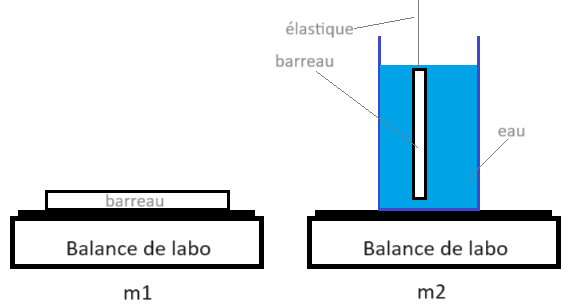
\includegraphics{doublePesee.png}}
    \caption{Double pesée}
\end{figure}\\
Il suffit ensuite d'appliquer la formule (23)
\newpage

\paragraph{Equations physiques}
\begin{align}
    \intertext{Masse volumique par la méthode de la double pesée : }
    \rho &= \rho_{l} \frac{m_{1} }{m_{2}}\\
    \shortintertext{ $\rho_{l} : $ masse volumique du liquide $[\frac{kg}{m^3}]$}
    \shortintertext{ $m_{1} : $ masse $[kg]$ }
    \shortintertext{ $m_{2} : $ masse immergée $[kg]$ } \notag
\end{align}
\begin{align}
    \intertext{Equation de d'Alembert sur l'axe Ox:}
    \frac{\partial^2 \xi}{\partial x^2} &= \frac{1}{c^2} \frac{\partial^2 \xi}{\partial t^2}\\
    \shortintertext{ $\xi : $ Gandeur physique portant l'onde $[\frac{[\xi]}{m^2}]$}
    \shortintertext{ $c : $ vitesse de propagation de l'onde $[\frac{m}{s}]$ }\notag
\end{align}
Ondes longitudinales dans un barreau solide ~\cite{Polycop-Ondes} :
\begin{figure}[h]
    \centering
    \adjustbox{max width=\textwidth}{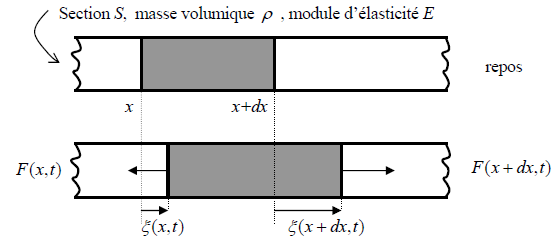
\includegraphics{OndesLongBarreauSol.png}}
    \caption{Barreau.~\cite{Polycop-Ondes}}
\end{figure}
\begin{align}
    \sigma(x,t)=\frac{F(x,t)}{S} &= E \frac{allongement}{longueur au repos} \notag \\
    &= E \frac{\xi(x+dx,t)-\xi(x,t)}{dx}\\
    \intertext{On peut en déduire l'équation de l'onde dans un barreau solide}
    \frac{\partial^2 \xi}{\partial x^2} &= \frac{\rho}{E} \frac{\partial^2 \xi}{\partial t^2}\\
    \shortintertext{ $\rho : $ masse volumique $[\frac{kg}{m^3}]$}
    \shortintertext{ $E : $ module d'élasticité du solide $[GPa]$}
    \intertext{Equation comparant l'équation de l'onde et celle de d'Alembert on obtient la propagation
     des ondes sinusoïdales dans les milieux solides (Equation 14) :}
    c &= \sqrt{\frac{E}{\rho}} \notag \\
    \implies E &= c^2 \rho 
    \shortintertext{ $c : $ vitesse de propagation de l'onde $[\frac{m}{s}]$}\notag
\end{align}
%\paragraph{Liste des paramètres}
%\begin{itemize}
 %   \item $\rho : $ masse volumique du matériel $[\frac{kg}{m^3}]$
  %  \subitem $m_{1} : $masse $[kg]$
   % \subitem $m_{2} : $masse immergée $[kg]$
    %\subitem $\rho_{l} : $masse volumique du liquide $[\frac{kg}{m^3}]$
%    \item $E : $module le Young du matériel $[Pa]$
 %   \item $v : $vitesse de propagation de l'onde $[\frac{m}{s}]$
%\end{itemize}
\paragraph{Calculs d'incertitudes}
La propagation d'incertitude basée sur le cours IPH est calculé de la manière 
suivante:~\cite{gravier-laurent}\\[2ex]
\begin{align}
    \intertext{Masse volumique : }
    \frac{\Delta \rho}{\rho} &= \frac{\Delta \rho_{l}}{\rho_{l}} + \frac{\Delta m_{1}}{m_{1}} + \frac{\Delta m_{2}}{m_{2}}\\
    \intertext{Module de Young : }
    \frac{\Delta E}{E} &= 2 \frac{\Delta c}{c} + \frac{\Delta \rho}{\rho}
\end{align}
\subsubsection{\large Protocole expérimental}
\begin{enumerate}
    \item Mesure de la masse volumique d'au moins 3 matériaux. 
    \subitem Suivant la méthode de la double pesée d'Archimède exprimée plus haut (équation 18). 
    \item Mesure de la longueur des barreaux au pied à coulisse
    \item Mise en résonance des différents barreaux sur notre montage expérimental pour en déduire la 
    vitesse de propagation du son dans le matériel
    \item Calcul avec leurs incertitudes des modules de Young des différents matériaux
\end{enumerate}

\paragraph{Présentation du montage}
Le montage utilisé pour la mesure de la vitesse de déplacement du son est exactement le 
même que dans les expérimentations précédentes.\\
Pour la mesure de la masse volumique, la méthode de la double pesée d'Archimède est utilisée. Le 
schéma est dans les rappels théoriques (Figure 5). %%%%% modifier numero 
Un élastique est utilisé pour accrocher le barreau à mesurer et le support de laboratoire. Il a l'avantage
de directement adhérer à la surface du barreau ce qui évite de devoir percer notre échantillon et 
fausser la mesure de la célérité. Son volume immergé et sa masse sont faibles et ne fausseront pas 
significativement nos mesures. Pour les matériaux dont la densité est plus faible que celle de l'eau, 
ils seront immergés à l'aide d'une fine pointe. De la même manière que pour l'élastique, les faibles
masse et volume de l'outil ne fausseront pas significativement nos résultats. 
\paragraph{Liste du matériel}
Mesures de la vitesse de propagation du son :\\
Le matériel utilisé est le même qu'à la manipulation précédente.\\
Mesure de la masse volumique :
\begin{itemize}
    \item Balance de laboratoire
    \item Long récipiant pour l'eau
    \item Supports de laboratoire
    \item Elastique
    \item Pointe fine
\end{itemize}
\paragraph{Méthode de mesure}
La méthode de mesure pour calculer la vitesse de propagation de l'onde $c$ est la même que pour 
l'expérimentation précédente.\\
Pour les masses, mesurées grâce à la balance de laboratoire, et les longueurs, mesurée au pied à 
coulisse les incertitudes sont calculées en fonction du nombre de chiffres significatif affiché sur 
l'appareille de mesure. \\
La masse volumique, calculé avec la méthode de la double pesée d'Archimède, l'incertitude est 
calculée suivant l'équation 29. L'incertitude relative de la masse volumique de l'eau sera de 0.5 pourcent
pour une valeur $\rho_{eau}=998[\frac{kg}{m^3}]$, car elle varie selon les conditions de température 
et de pression. Nous réaliserons les mesures de vitesses de 
propagation du son dans le but de calculer les modules de Young dans des
barreaux solides 
d'au moins 3 matériaux différents.

\newpage

\subsection{\large Résultats / Analyse}
\subsubsection{\large Données brutes}
\paragraph{\large Cylindre Aluminium 100 mm}
\paragraph{Tableau}
\paragraph{Graphe}
\paragraph{Observations}

\paragraph{\large Cylindre Acier inox 200 mm}
\paragraph{Tableau}
\paragraph{Graphe}
\paragraph{Observations}

\paragraph{\large Cylindre Acier inox 400 mm}
\paragraph{Tableau}
\paragraph{Graphe}
\paragraph{Observations}

\newpage

\subsubsection{\large Données réduites}
\paragraph{\large Cylindre Acier inox 100 mm}
\paragraph{Calculs}
\paragraph{Incertitudes}

\paragraph{\large Cylindre Acier inox 200 mm}
\paragraph{Calculs}
\paragraph{Incertitudes}

\paragraph{\large Cylindre Acier inox 400 mm}
\paragraph{Calculs}
\paragraph{Incertitudes}

\newpage

\subsubsection{\large Tableau récapitulatif}
\paragraph{Valeurs}
\paragraph{Incertitudes relatives}
\paragraph{Ecart relatif}

\subsubsection{\large Discussion quantitative}
\paragraph{Incertitude > écart}
validation
\paragraph{Incertitude < écart}
invalidation
discussion critique des méthodes